\section{Introduction}
One of the goals of the thesis is to design and implement a scalable electronic voting application. As software engineers our focus is on the software architecture and we will follow the definition from Bass et al. \cite{Bass}. 


%**************************************Definition Software architecture
\begin{defi}[\textbf{Software architecture}]
The software architecture of a system is the set of \textbf{structures} needed to reason about the system, which comprise software \textbf{elements}, \textbf{relations} among them, and the \textbf{properties} of both.  \cite{Bass}
\end{defi}
%**************************************Definition Software architecture End

\noindent
Our approach towards implementing a software architecture is based on a systematic analysis of the demands for the application. To achieve this we will use methods and techniques from previous causes in Software architecture such as  Quality attribute workshop, Quality attribute scenario (QAS) and architectural decisions etc. A quality attribute (QA) according to Bass et al. is as follows.


%**************************************Definition Quality attribute
\begin{defi}[\textbf{Quality attribute}]
..A quality attribute is a measurable or testable property of a system that is used to indicate how well the satisfies the needs of its stakeholders..  \cite{Bass}
\end{defi}
%**************************************Definition Quality attribute End

\noindent
A core observation is that a QA should be measurable or testable quality. The key point is when working with QA we use them in a given context/scenario and therefor we informally call these as QAS.\\


\begin{figure}[H]
\centering
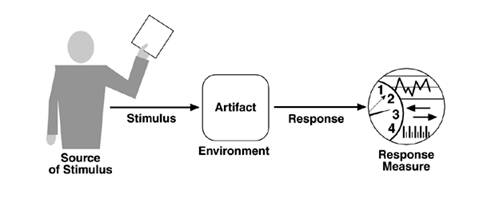
\includegraphics[scale=0.8]{QualityAttributeScenario.jpg}

\caption{The parts of a quality attribute scenario}
\label{fig:Quality_Attribute_Scenario}
\end{figure}





\noindent
One of the core aspects of the definition of software architecture, is that software architecture is a set of structures, which we can use to reason about the system. To assist and visualize these structures, elements, relations and properties we use Module-, Component \& Connector (C\&C)- and Allocation viewpoints \cite{3+1}. 

\begin{enumerate}
    \item Module viewpoint is concerned with how functionality of the system maps to static development units. The focus will be on elements such as classes and interfaces and relationships such as associations, generalizations, realizations and dependencies.
    \item Component \& Connector viewpoint is concerned with the runtime mapping of functionality to components of the architecture. Components are the executing things that perform a function. Connectors are the communication channels between components. The purpose is to focus on the flow of data and responsibilities such as a network call or method call etc.
    \item Allocation viewpoint is concerned with how software entities are mapped to environmental entities. Here the focus are on the physical stuff such as computer or a network. We specify the environment in order to make the software running. 
\end{enumerate}

\noindent
These viewpoint originates from $3+1$ article \cite{3+1}, where the $+1$ is the architectural requirements. These architectural requirements can be formulated through QAS.\\

\noindent
We will discuss different tactics on software architecture for achieving the business goal for the electronic voting application. A tactic according to Bass et al. is defined as.

%**************************************Definition Tactic
\begin{defi}[\textbf{Tactic}]
Tactic is a design decision that influences the achievement of a quality attribute response. \cite{Bass}
\end{defi}
%**************************************Definition Tactic End

\noindent
We will introduce a case which gives an overall description of how a user creates a vote through an electronic voting application. The purpose of the case is describing business/mission requirement of the electronic voting application. Here we will emphasize that it should be clear it reflects the security requirements from the first part. We use the general security requirement for an electronic voting scheme described in chapter 2 as functional requirements for the application. These requirements are well studied and discussed and should be comprehensive for an electronic voting scheme.